\chapter{Algoritmos Voraces (Greedy)}

\section{Introducción}

Los algoritmos voraces son aquellos que resuelven problemas de optimización, es decir, problemas en los que se busca encontrar la mejor solución entre todas las posibles. La idea de estos algoritmos es ir tomando decisiones en cada paso, eligiendo la opción que parece ser la mejor en ese momento, sin importar las consecuencias a futuro. En general, los algoritmos voraces son fáciles de implementar y de entender, pero no siempre encuentran la solución óptima.

\section{Forma general}

\begin{codebox}{Forma general de un algoritmo voraz}
\begin{pascallike}
fun voraz(C:Set of "Candidato") ret S : "Solucion a construir"
	S := "solucion vacia"
	do S "no es solucion" -> 
		c := "seleccionar" de C
		elim(C,c)
		if "agregar c a S es factible" then
			"agregar c a S"
		fi
	od
end fun
\end{pascallike}    
\end{codebox}

\begin{itemize}
    \item Inicialmente ningún candidato ha sido considerado, es decir, ni incorporado ni descartado.
    \item En cada paso se utiliza la función de \textbf{selección} para elegir cuál candidato considerar.
    \item Se chequea que el candidato considerado sea factible para incorporarlo a la solución y se lo agrega o no.
    \item Se repiten los pasos anteriores hasta que la colección de candidatos elegidos sea una solución.
\end{itemize}

\section{¿Cómo saber si un problema admite una solución voraz?}

\begin{itemize}
    \item \textbf{Principio de la elección voraz:} Seleccionar la opción que parece ser la mejor en ese momento.
    \item \textbf{Subestructura óptima:} La solución óptima al problema contiene la solución óptima a los subproblemas.
    \item \textbf{Greedy-choice property:} Una secuencia de decisiones es voraz si se puede tomar la primera decisión sin importar las consecuencias futuras.
\end{itemize}

\section{Problemas resueltos con algoritmos voraces}

\subsection{Problema de la moneda}

\begin{itemize}
    \item Se tiene un conjunto de monedas de diferentes valores y se busca dar un cambio de $n$ unidades de dinero.
    \item Se busca minimizar la cantidad de monedas a utilizar.
\end{itemize}

La forma de seleccionar va a se \textbf{tomar una moneda de la mayor denominación posible que no exceda el monto a pagar, utilizar exactamente el mismo algoritmo para el importe remanente.}

\begin{codebox}{Algoritmo de la moneda v1}
\begin{pascallike}
fun cambio(m: Nat, C: Set of Nat) ret S : Nat
    var c, resto: Nat
    var C_aux : Set of Nat
    S:= 0
    C_aux:= set_copy(C)
    resto:= m
    do resto > 0 $\rightarrow$
        c := seleccion(C_aux,resto)
        elim(C_aux,c)
        S := S + resto div c
        resto := resto mod c
    od
    set_destroy(C_aux)
end fun
\end{pascallike}
\end{codebox}

\begin{codebox}{Algoritmo de la moneda v2}
\begin{pascallike}
fun cambio(m: Nat,C: Set of Nat) ret S : Nat
    var c, resto: Nat
    var C_aux : Set of Nat
    S:= 0
    C_aux:= set_copy(C)
    resto:= m
    do (not is_empty_set(C_aux)) $\rightarrow$
        c := seleccion(C_aux,resto)
        if c > resto {-chequeo factibilidad-}
            then elim(C_aux,c)
            else resto := resto - c
            S := S + 1 
        fi
    od
    set_destroy(C_aux)
end fun
\end{pascallike}
\end{codebox}


\subsection{Problema de la mochila}

\begin{itemize}
    \item Se tiene una mochila de capacidad $W$, y $n$ objetos de valor $v_i$ y peso $w_i$.
    \item Se busca llenar la mochila con los objetos de manera que se maximice el valor total de los objetos.
    \item Por mejor selección, se entiende que se elige el objeto con mayor valor por unidad de peso sin exceder la capacidad de la mochila.
    \item Para que la solucion no sea trivial, se debe cumplir que la suma de los pesos de los objetos sea mayor a la capacidad de la mochila.
\end{itemize}

\begin{enumerate}
    \item \textbf{Primer Criterio de selección posible:} tomar el objeto con mayor valor por unidad de peso.
    \begin{itemize}
        \item \textit{Razonabilidad}: el objetivo es cargar la mochila con el mayor valor posible, escogemos los objetos más valiosos.
        \item \textit{Falla}: puede que al elegir un objeto valioso dejemos de lado otro apenas menos valioso pero mucho más liviano.
    \end{itemize}
    \item \textbf{Segundo Criterio de selección posible:} tomar el objeto con menor peso.
    \begin{itemize}
        \item \textit{Razonabilidad}: hay que procurar aprovechar la capacidad de la mochila, escogemos los objetos más livianos.
        \item \textit{Falla}: puede que al elegir un objeto liviano dejemos de lado otro apenas más pesado pero mucho más valioso.
    \end{itemize}
    \item \textbf{Tercer Criterio de selección posible:} la combinación de los dos anteriores.
    \begin{itemize}
        \item Debemos asegurarnos de que cada kg utilizado de la mochila sea aprovechado de la mejor manera posible: que cada kg colocado en la mochila valga lo más posible.
        \item Criterio: elegir el de mayor valor relativo (cociente entre el valor y el peso): dicho cociente expresa el valor promedio de cada kg de ese objeto.
        \item Falla: puede que al elegir un objeto dejemos de lado otro de peor cociente, pero que aprovecha mejor la capacidad.
    \end{itemize}
\end{enumerate}

\textbf{El problema de la mochila no admite solución voraz.} Se simplifica permitiendo fraccionar elementos.

\begin{codebox}{Algoritmo de la mochila fraccionaria}
\begin{pascallike}
type Objeto = tuple
                id : Nat
                value: Float
                weight: Float
            end tuple

type Obj_Mochila = tuple
                    obj : Objeto
                    fract : Float
                end tuple

fun mochila(W: Float, C: Set of Objeto) ret L : List of Obj_Mochila
    var o_m : Obj_Mochila var resto : Float
    var C_aux : Set of Objeto
    S:= empty_list()
    C_aux:= set_copy(C)
    resto:= W
    do (resto > 0) $\rightarrow$
        o_m.obj := select_obj(C_aux)
        if o_m.obj.weight <= resto
            then o_m.fract := 1.0
                resto := resto - o_m.obj.weight
            else o_m.fract := resto/o_m.obj.weight
                resto := 0
        fi
        addl(S,o_m)
        elim(C_aux,o_m.obj)
    od
    set_destroy(C_aux)
end fun
\end{pascallike}
\end{codebox}

\section{Algoritmos voraces en grafos}

\subsection{Árbol generador de costo mínimo}

\begin{itemize}
    \item Se tiene un grafo conexo con pesos en las aristas.
    \item Se busca un árbol generador que contenga todos los vértices y cuya suma de pesos de las aristas sea mínima.
\end{itemize}

\subsubsection{Ejemplo}
Se tiene el siguiente grafo y se busca un árbol generador de costo mínimo.
\begin{figure}[h]
    \centering
    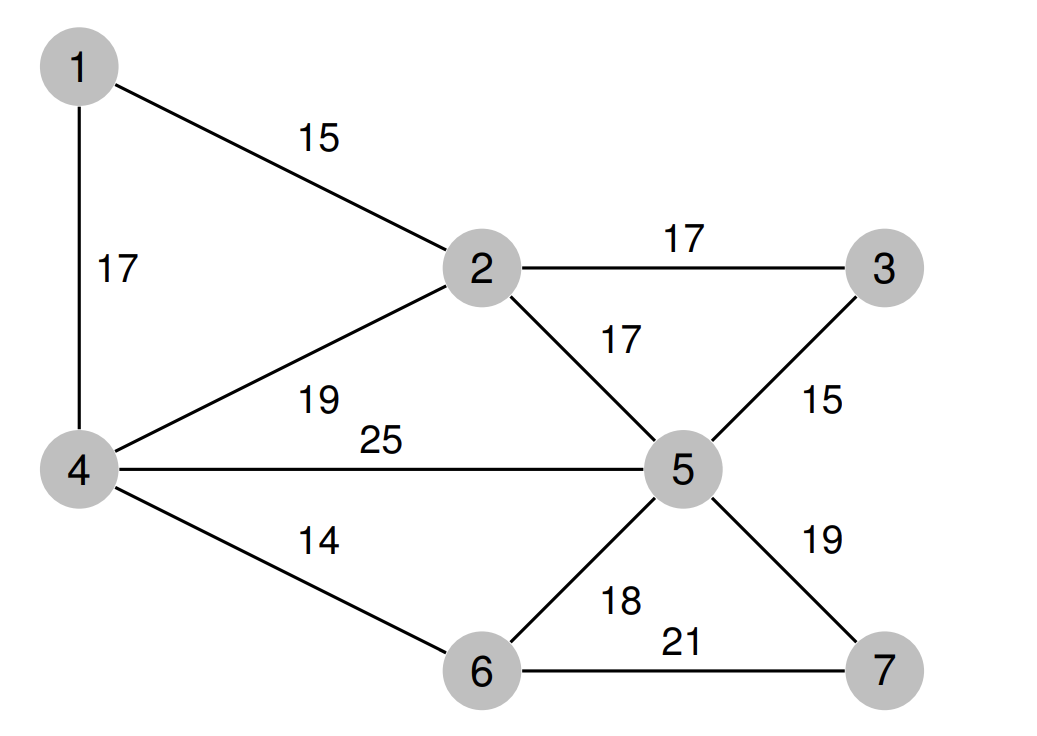
\includegraphics[scale=0.5]{estáticos/figura6.png}
\end{figure}
El algoritmo de Prim es un algoritmo perteneciente a la teoría de los grafos para encontrar un árbol recubridor mínimo en un grafo conexo, no dirigido y cuyas aristas están etiquetadas.

En otras palabras, el algoritmo encuentra un subconjunto de aristas que forman un árbol con todos los vértices, donde el peso total de todas las aristas en el árbol es el mínimo posible. Si el grafo no es conexo, entonces el algoritmo encontrará el árbol recubridor mínimo para uno de los componentes conexos que forman dicho grafo no conexo.

En este caso se utiliza de la siguiente manera:
\begin{enumerate}
    \item Parte desde el vértice 6,
    \item Selecciona la arista de menor peso que conecta el árbol con un vértice no incluido en el árbol. Selecciona la arista que une al 6 con el 4,
    \item Selecciona la arista de menor peso que conecta el árbol con un vértice no incluido en el árbol. Selecciona la arista que une al 4 con el 1,
    \item  Selecciona la arista de menor peso que conecta el árbol con un vértice no incluido en el árbol. Selecciona la arista que une al 1 con el 2,
    \item  Selecciona la arista de menor peso que conecta el árbol con un vértice no incluido en el árbol. Selecciona la arista que une al 2 con el 5,
    \item  Selecciona la arista de menor peso que conecta el árbol con un vértice no incluido en el árbol. Selecciona la arista que une al 5 con el 3.
    \item  Selecciona la arista de menor peso que conecta el árbol con un vértice no incluido en el árbol. Selecciona la arista que une al 5 con el 7.
\end{enumerate}

\begin{figure}[h]
    \centering
    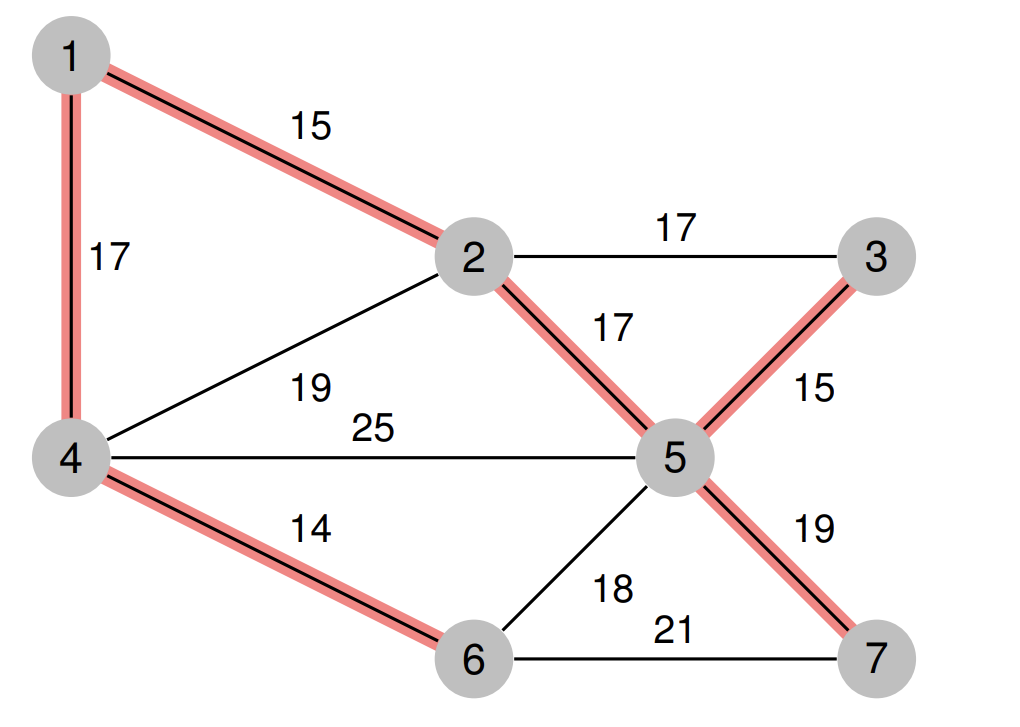
\includegraphics[scale=0.5]{estáticos/figura7.png}
\end{figure}

\begin{codebox}{Algoritmo de Prim}
\begin{pascallike}
type Vertex = Nat

type Edge = tuple
                v1 : Vertex
                v2 : Vertex
                cost : Nat
            end tuple

type Graph = tuple
                vertices : Set of Vertex
                edges : Set of Edge
            end tuple

fun Prim(G : Graph, k: Vertex) ret T: Set of Edge
    var c: Edge
    var C: Set of Vertex
    C:= copy_set(G.vertices)
    elim(C,k)
    T:= empty_set()
    do (not is\_empty\_set(C)) $\rightarrow$
        c := seleccionarArista(G.edges,C)
        if member(c.v1,C) then 
            elim(C,c.v1)
        else elim(C,c.v2)
        add(T,c)
        fi
    od
end fun
\end{pascallike}
\end{codebox}

\subsection{Camino de costo mínimo}

\begin{itemize}
    \item Se tiene un grafo conexo con pesos en las aristas.
    \item Se busca un camino que una dos vértices y cuya suma de pesos de las aristas sea mínima.
\end{itemize}

\subsubsection{Dijkstra}
El algoritmo de Dijkstra, también llamado algoritmo de caminos mínimos, es un algoritmo para la determinación del camino más corto, dado un vértice origen, hacia el resto de los vértices en un grafo que tiene pesos en cada arista. Su nombre alude a Edsger Dijkstra, científico de la computación de los Países Bajos que lo describió por primera vez en 1959.

La idea subyacente en este algoritmo consiste en ir explorando todos los caminos más cortos que parten del vértice origen y que llevan a todos los demás vértices; cuando se obtiene el camino más corto desde el vértice origen hasta el resto de los vértices que componen el grafo, el algoritmo se detiene. Se trata de una especialización de la búsqueda de costo uniforme y, como tal, no funciona en grafos con aristas de coste negativo (al elegir siempre el nodo con distancia menor, pueden quedar excluidos de la búsqueda nodos que en próximas iteraciones bajarían el costo general del camino al pasar por una arista con costo negativo).

Suponga que se tiene el siguiente grafo y se busca el camino de costo mínimo.
\begin{figure}[h]
    \centering
    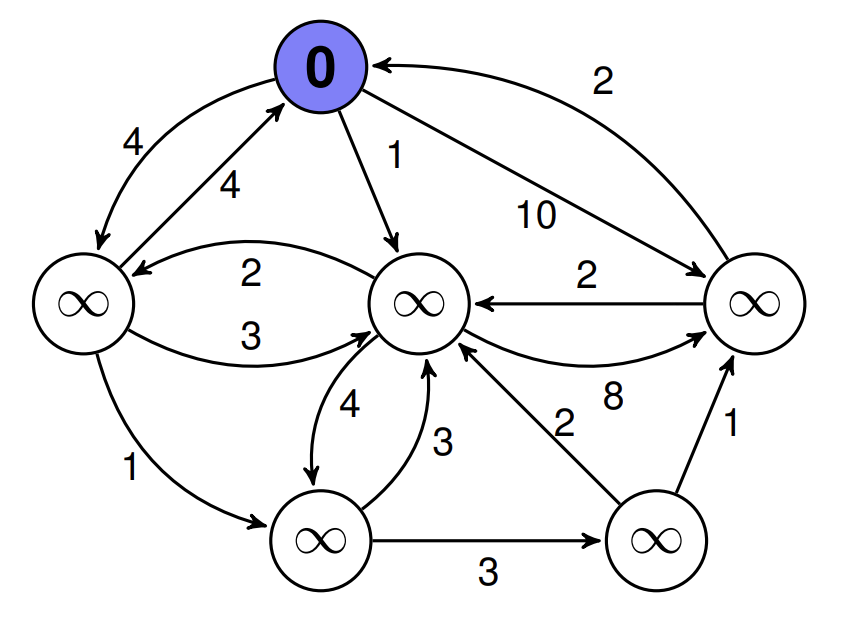
\includegraphics[scale=0.5]{estáticos/figura8.png}
\end{figure}

\begin{enumerate}
    \item Parte desde el vértice seleccionado, y actualiza los valores de los vértices adyacentes, y selecciona el de menor costo. La seleccion va $(0,1)$
    \item  Actualiza los valores de los vértices adyacentes, y selecciona el de menor costo $(0,1,3)$,
    \item  Actualiza los valores de los vértices adyacentes, y selecciona el de menor costo $(0,1,3,4)$,
    \item  Actualiza los valores de los vértices adyacentes, y selecciona el de menor costo $(0,1,3,4,7)$,
    \item  Actualiza los valores de los vértices adyacentes, y selecciona el de menor costo $(0,1,3,4,7,8)$,
    \item El algoritmo termina. No hay más vértices por visitar.
\end{enumerate}
\newpage
\begin{figure}[h]
    \centering
    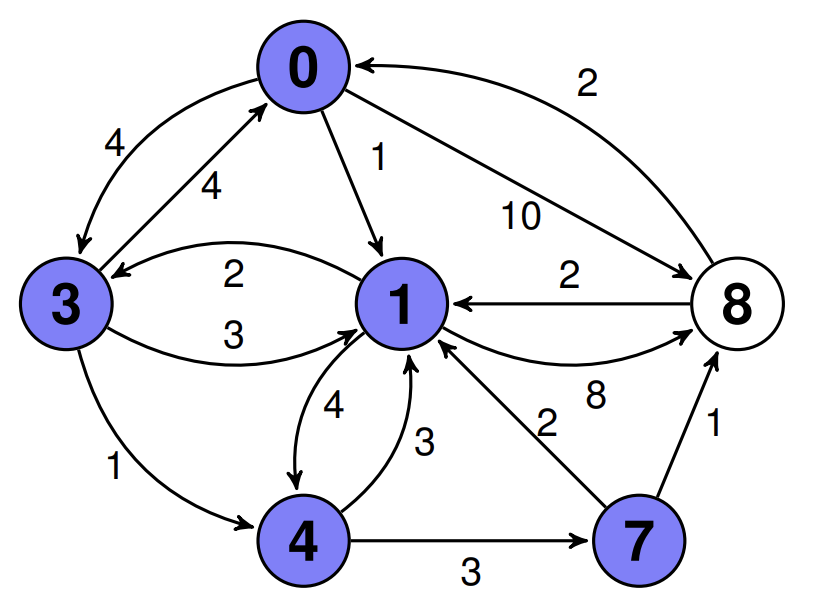
\includegraphics[scale=0.5]{estáticos/figura9.png}
\end{figure}

\begin{codebox}{Algoritmo de Dijkstra}
\begin{pascallike}
fun Dijkstra(L: array[1..n,1..n] of Nat, v: Nat) ret D: array[1..n] of Nat
    var c: Nat
    var C: Set of Nat
    for i := 1 to n do add(C,i) od
    elim(C,v)
    for j:= 1 to n do D[j]:= L[v,j] od
    do (not is_empty_set(C)) $\rightarrow$
        c:= seleccion(C,D)
        elim(C,c)
        for j in C do D[j]:= min(D[j],D[c]+L[c,j]) od
    od
end fun
\end{pascallike}
\end{codebox}

\begin{itemize}
    \item Se inicializa un conjunto $C$ con todos los vértices del grafo, excepto el vértice origen.
    \item Se inicializa un arreglo $D$ con las distancias desde el vértice origen a cada uno de los vértices del grafo.
    \item Se selecciona el vértice $c$ tal que $D[c]$ sea mínimo.
    \item Se elimina el vértice $c$ del conjunto $C$.
    \item Se actualizan las distancias de los vértices adyacentes a $c$.
    \item Se repiten los pasos anteriores hasta que el conjunto $C$ sea vacío.
\end{itemize}
    